% Supporting Information for the SciencePG submission.
\documentclass[11pt,a4paper]{article}
\usepackage[margin=2.5cm]{geometry}
\usepackage{times}
\usepackage{amsmath,amssymb}
\usepackage{booktabs}
\usepackage{graphicx}
\graphicspath{{./}}
\usepackage[labelsep=period, labelfont=bf, font=small, font=it]{caption}
\renewcommand{\thetable}{S\arabic{table}}
\renewcommand{\thefigure}{S\arabic{figure}}
\begin{document}
\begin{center}
{\Large\bfseries Supporting Information}\\[6pt]
{\large A Reproducible Event-Fixed Protocol for Evaluating Financial Stress Detectors}\\[4pt]
Prashant Singh, Pranav Singh\\
Department of Mathematics, Indian Institute of Technology Ropar, Rupnagar, India
\end{center}

\noindent This file collects the sensitivity and ablation material referenced from the
main text: event-window sensitivity (Table~S1, Figure~S1), the composite
weight ablation (Table~S2), the sign-convention ablation for the persistence
statistic (Table~S3), and the confirmation-window sensitivity (Figure~S2).
All values are produced by the reproducibility package accompanying the
article.

\begin{table}[htbp]
\centering
\caption{Event-window sensitivity for pointwise precision, recall, F1, and FPR.}
\label{tab:eventwindow}
\scriptsize
\begin{tabular}{llrrrr}
\toprule
Window & Method & Prec. & Recall & F1 & FPR\\
\midrule
$\pm20$ & Vol. & 0.390 & 0.396 & 0.393 & 0.061\\
$\pm20$ & Hybrid & 0.545 & 0.216 & 0.309 & 0.018\\
$\pm30$ & Vol. & 0.499 & 0.344 & 0.407 & 0.052\\
$\pm30$ & Hybrid & 0.692 & 0.186 & 0.293 & 0.012\\
$\pm45$ & Vol. & 0.571 & 0.266 & 0.363 & 0.048\\
$\pm45$ & Hybrid & 0.815 & 0.148 & 0.251 & 0.008\\
$\pm60$ & Vol. & 0.640 & 0.225 & 0.333 & 0.044\\
$\pm60$ & Hybrid & 0.886 & 0.122 & 0.214 & 0.005\\
\bottomrule
\end{tabular}
\end{table}

\begin{figure}[htbp]
\centering
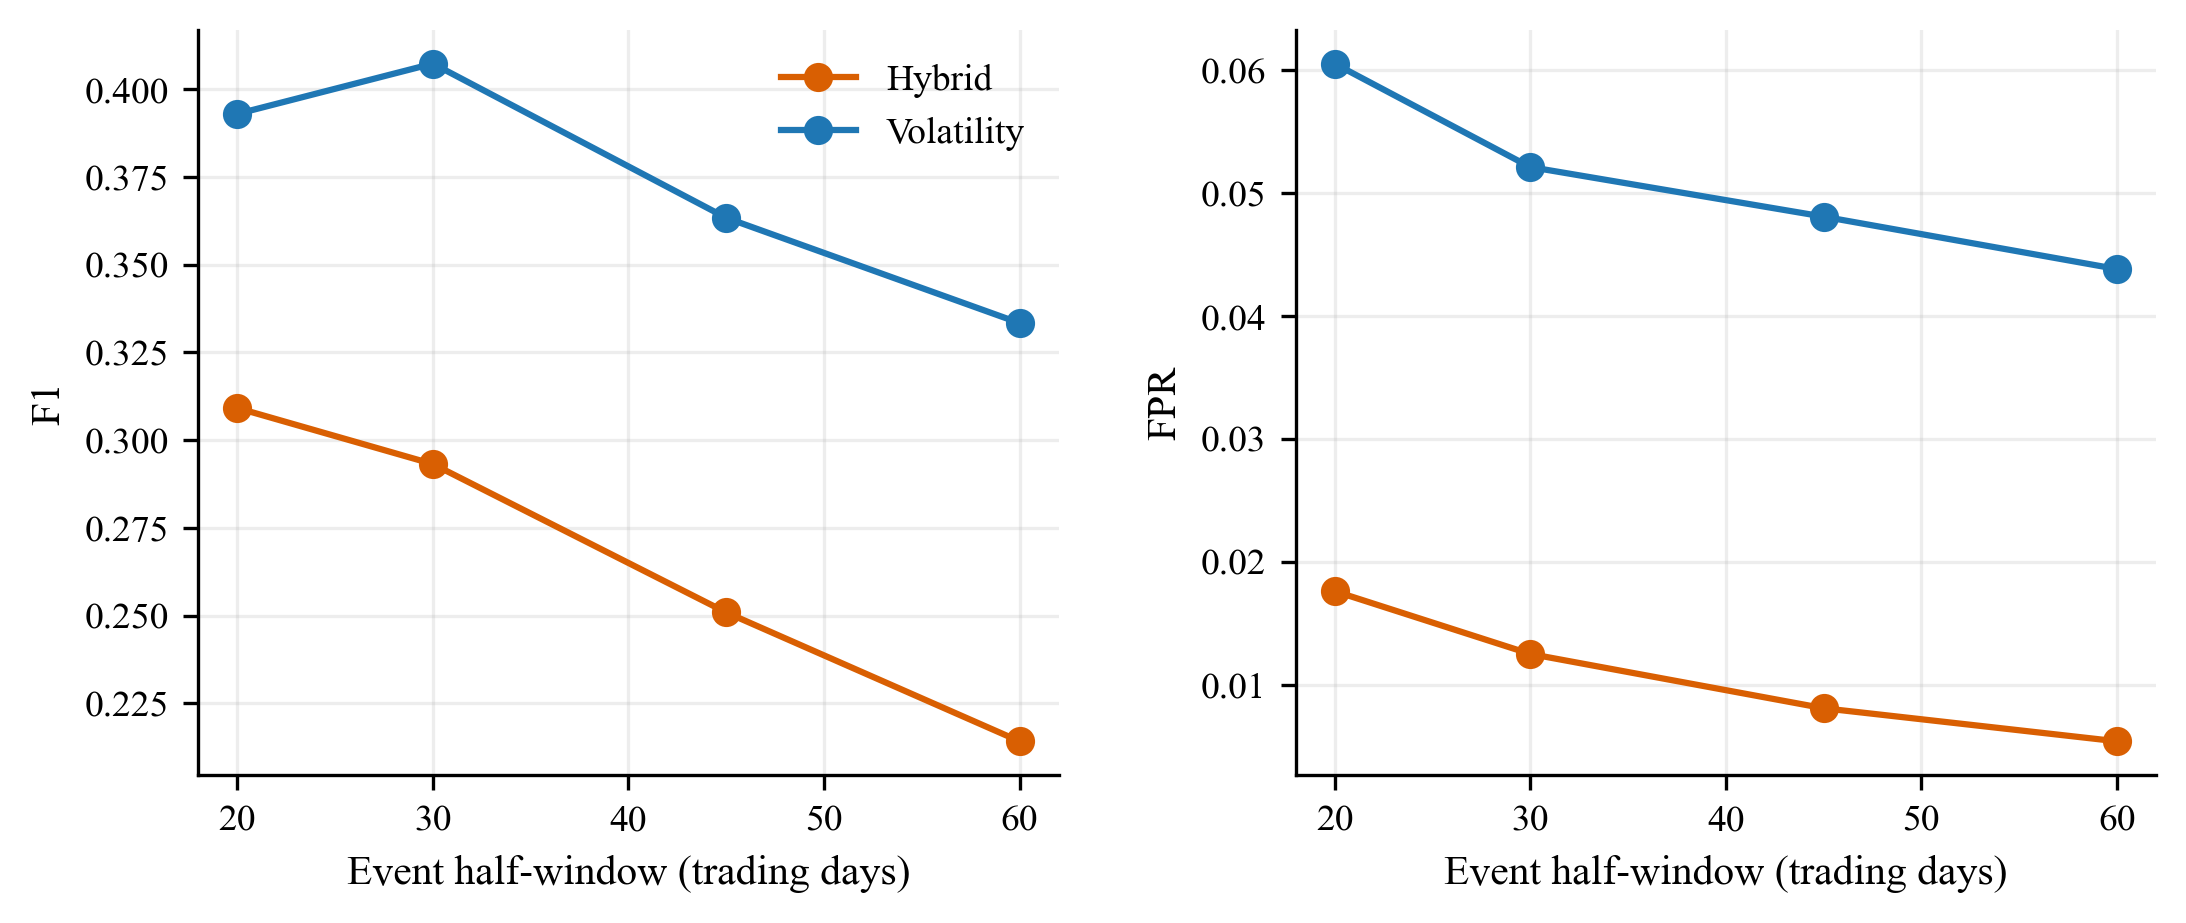
\includegraphics[width=0.95\linewidth]{event_window_sensitivity.png}
\caption{Event-window sensitivity across $\pm20$, $\pm30$, $\pm45$, and $\pm60$ trading-day windows.}
\label{fig:eventwindow}
\end{figure}

\begin{table}[htbp]
\centering
\caption{Composite weight ablation. Each row recomputes $x_t$, the MMD and $\kappa$ components, and the hybrid. Events are counted out of 13.}
\label{tab:weights}
\scriptsize
\begin{tabular}{lrrrrrr}
\toprule
$(w_r,w_\sigma,w_z)$ & Prec. & Recall & F1 & FPR & Delay & Events\\
\midrule
$(0.5,0.3,0.2)$ default & 0.886 & 0.122 & 0.214 & 0.005 & 6.8 & 8\\
$(1/3,1/3,1/3)$ equal & 0.886 & 0.122 & 0.214 & 0.005 & 6.8 & 8\\
$(0.2,0.3,0.5)$ reversed & 0.886 & 0.122 & 0.214 & 0.005 & 6.8 & 8\\
$(0.6,0.2,0.2)$ & 0.882 & 0.122 & 0.214 & 0.006 & 6.8 & 8\\
$(0.4,0.4,0.2)$ & 0.886 & 0.122 & 0.214 & 0.005 & 6.8 & 8\\
$(0.5,0.2,0.3)$ & 0.886 & 0.122 & 0.214 & 0.005 & 6.8 & 8\\
$(0.2,0.6,0.2)$ & 0.900 & 0.135 & 0.235 & 0.005 & 4.4 & 8\\
$(1,0,0)$ returns only & 0.845 & 0.131 & 0.227 & 0.008 & 0.8 & 8\\
$(0,1,0)$ volatility only & 0.815 & 0.121 & 0.210 & 0.009 & 1.4 & 7\\
$(0,0,1)$ z-score only & 0.886 & 0.122 & 0.214 & 0.005 & 6.8 & 8\\
\bottomrule
\end{tabular}
\end{table}

\begin{table}[htbp]
\centering
\caption{Confirmation-term ablation for the persistence statistic. The low-$\kappa$ variant is the direction predicted by critical-slowing-down theory.}
\label{tab:kappasign}
\scriptsize
\begin{tabular}{lrrrrrr}
\toprule
Confirmation term & Prec. & Recall & F1 & FPR & Delay & Events\\
\midrule
$|z_\kappa|$ two-sided (default) & 0.886 & 0.122 & 0.214 & 0.005 & 6.8 & 8\\
$\max(-z_\kappa,0)$ low $\kappa$ & 0.875 & 0.114 & 0.202 & 0.006 & 6.7 & 7\\
$\max(+z_\kappa,0)$ high $\kappa$ & 0.874 & 0.141 & 0.242 & 0.007 & 1.6 & 7\\
\bottomrule
\end{tabular}
\end{table}

\begin{figure}[htbp]
\centering
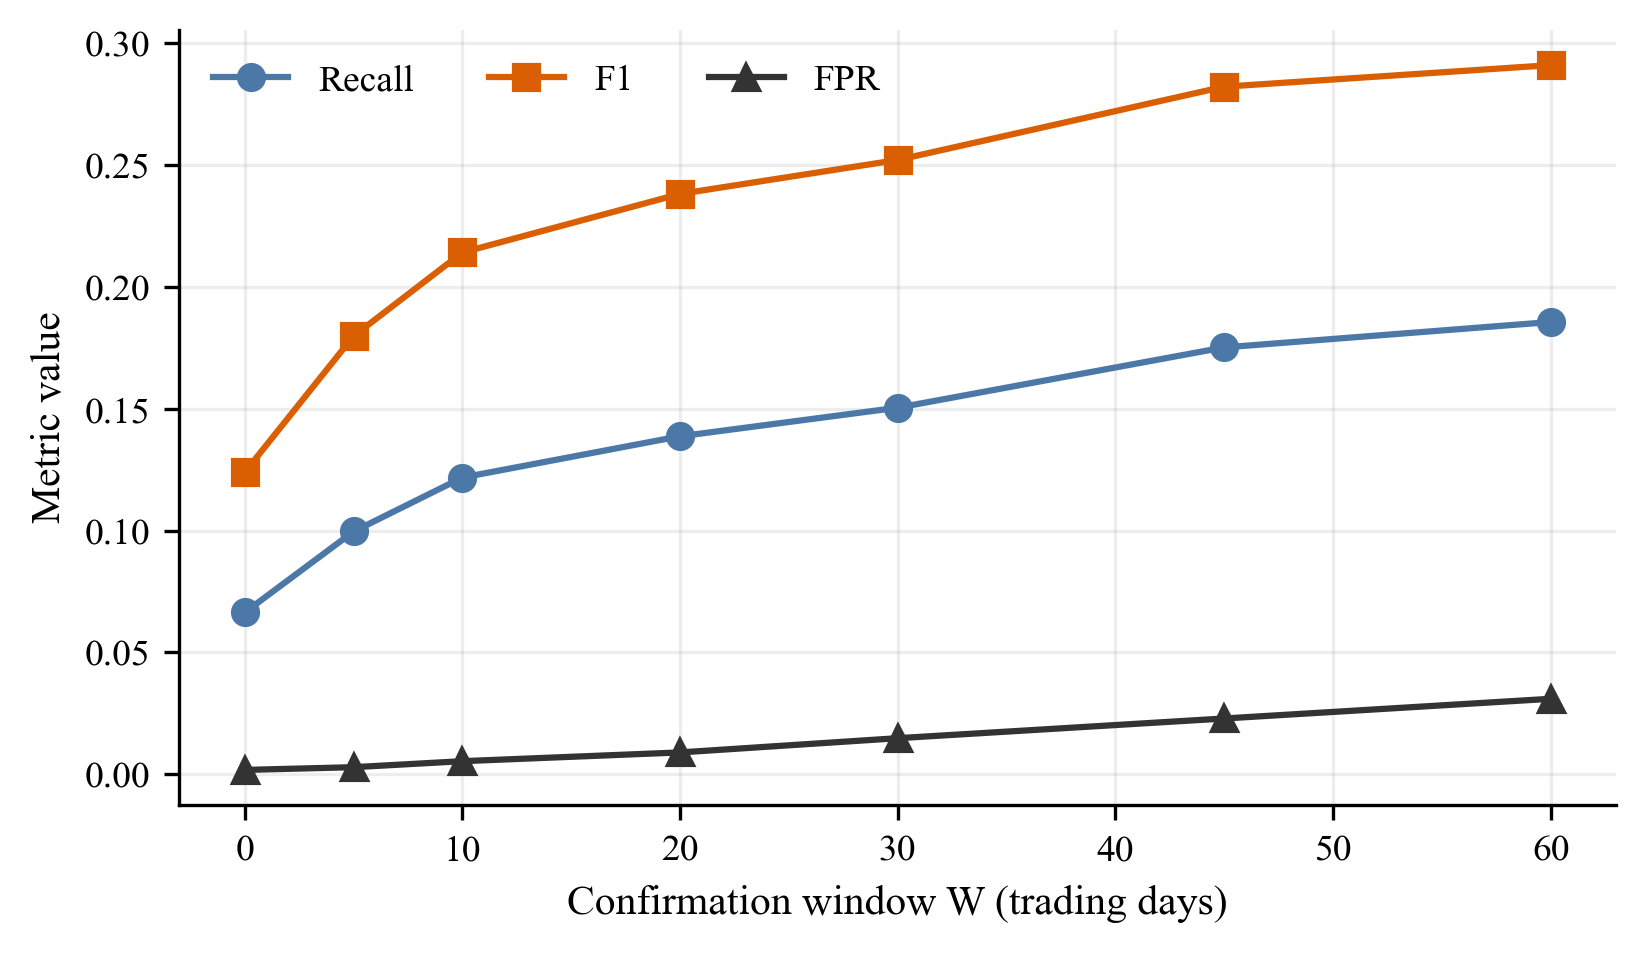
\includegraphics[width=0.75\linewidth]{confirmation_window_sensitivity.png}
\caption{Hybrid confirmation-window sensitivity showing how the retrospective confirmation window changes F1 and FPR.}
\label{fig:window_sensitivity}
\end{figure}

\end{document}
